% Author: Oliver Sheridan-Methven, December 2016.
% Documentation for various integer programming and linear programming
% solutions to the travelling salesman problem.
\documentclass[a4paper, 11pt]{article}

\usepackage{amsmath} % Nice maths symbols.
\usepackage{amssymb} % Nice variable symbols.
\usepackage{array} % Allow for custom column widths in tables.
\usepackage{arydshln} % Dashed lines using \hdashline \cdashline
\usepackage{bbm} % Gives Blackboard fonts.
\usepackage{bm} % Bold math symbols.
\usepackage[margin=10pt,font=small,labelfont=bf,labelsep=endash]{caption} % Caption figures and tables nicely.
\usepackage{enumitem} % Nice listing options in itemize and enumerate.
\usepackage{esdiff} % Gives nice differential operators.
\usepackage{esvect} % Gives nice vector arrows.
\usepackage{float} % Nice figure placement.
\usepackage{geometry} % Use nice margins.
\usepackage{graphicx} % Include figures.
\usepackage[colorlinks=true,linkcolor=blue,urlcolor=blue,citecolor=blue,anchorcolor=blue]{hyperref} % Colour links.
\usepackage{indentfirst} % Indents the first paragraph.
\usepackage{letltxmacro} % For defining a nice SQRT symbol.
\usepackage[framed,numbered,autolinebreaks,useliterate]{mcode} % Inports Listings package ideal for MATLAB.
\usepackage{multirow} % Nice table cells spanning many rows.
\usepackage{multicol} % If I want to use multiple columns.
\usepackage[numbers, sort&compress]{natbib} % Nice references.
\usepackage{physics} % Nice partial derivatives and BRAKET notation.
\usepackage{subcaption} % Side by side figures.
\usepackage{tabularx} % Tables with justified columns.
\usepackage{tikz} % For drawing pictures.


% Present the references in the order they are used.
\bibliographystyle{unsrtnat}

% Listing -> Code in environment labels.
\renewcommand{\lstlistingname}{Code}

% Nice paragraph indents.
\setlength{\parindent}{15mm}

% Giving the refereneces the right title. 
\renewcommand{\bibname}{References} 

% Gives nice margins.
\geometry{left=20mm, right=20mm, top=20mm, bottom=20mm}

% Removes hyphenation
\tolerance=1
\emergencystretch=\maxdimen
\hyphenpenalty=10000
\hbadness=10000

% To change the spacing in lists
%\setlist{noitemsep} % or \setlist{noitemsep} to leave space around whole list
\setenumerate{itemsep=-0.4em,topsep=0.5em} % Seems to look nice.

% Custom column widths using C{2cm}, L, R, etc.
\newcolumntype{L}[1]{>{\raggedright\let\newline\\\arraybackslash\hspace{0pt}}m{#1}}
\newcolumntype{C}[1]{>{\centering\let\newline\\\arraybackslash\hspace{0pt}}m{#1}}
\newcolumntype{R}[1]{>{\raggedleft\let\newline\\\arraybackslash\hspace{0pt}}m{#1}}

% Gives a nice column separation in multicolumn mode.
\setlength{\columnsep}{5mm}

% Figure environment for use in multicolumn. To put in captions use \captionof{figure}{content of caption}.
\newenvironment{Figure}
{\par\medskip\noindent\minipage{\linewidth}}
{\endminipage\par\medskip}

% Gives the nice SQRT symbol.
\makeatletter
\let\oldr@@t\r@@t
\def\r@@t#1#2{%
	\setbox0=\hbox{$\oldr@@t#1{#2\,}$}\dimen0=\ht0
	\advance\dimen0-0.2\ht0
	\setbox2=\hbox{\vrule height\ht0 depth -\dimen0}%
	{\box0\lower0.4pt\box2}}
\LetLtxMacro{\oldsqrt}{\sqrt}
\renewcommand*{\sqrt}[2][\ ]{\oldsqrt[#1]{#2}}
\makeatother

\begin{document}


\begin{center}
\begin{Large}
\textbf{Solving The Travelling Salesman Problem}\\
\end{Large}
\vspace{1ex}
\begin{large}
Oliver Sheridan-Methven 
\end{large}\\
December 2016 \\
\end{center}

\section*{Abstract}
We consider the travelling salesman problem for a set of 10 Spanish cities/provinces. We find a minimal round trip distance to be 2'999\:km. We compare the performance of some exact solvers, and various inexact faster solvers, suitable when exact solvers encounter memory/performance constraints. We implement algorithms using graph theory, integer programming, and linear programming.

\section{Introduction}

\subsection{Review of the travelling salesman problem}
\label{subsec:review_of_tsp}

There are multiple versions of the travelling salesman problem, each with small variations on what can constitute a solution. For clarity we state the problem as:
\begin{description}
\item[The travelling salesman problem] A salesman needs to travel to $ n $ cities, each of which are separated from each other by some positive nonzero distance. What route should the salesman take that has the minimal total distance such that they visit each and every city only once, returning to the starting city?
\end{description}


\subsection{Spanish cities}
\label{subsec:spanish_cities}

In order to test any algorithms and have a gauge of their performance, we consider the example set of Spanish cities with the  distance matrix in Table~\ref{tab:distance_matrix}. Notice that the distance matrix is symmetric. 

\begin{table}[hbt]
\begin{center}
\begin{tabular}{|l|cccccccccc|}
\cline{2-11}
\multicolumn{1}{c|}{} & Ali.   & Val.  & Bar. & Pam. & San. & Mad. & Sal. & Sev. & Mal.  & Gra. \\
\hline 
Alicante	& 0   & 515  & 353 & 422 & 482 & 673 & 634 & 815 & 609  & 166 \\
Valencia    & 515 & 0    & 868 & 621 & 997 & 437 & 778 & 693 & 1046 & 349 \\
Barcelona	& 353 & 868  & 0   & 434 & 129 & 841 & 631 & 827 & 256  & 519 \\
Pamplona	& 422 & 621  & 434 & 0   & 544 & 407 & 212 & 393 & 538  & 352 \\
Santander	& 482 & 997  & 129 & 544 & 0   & 951 & 756 & 937 & 219  & 648 \\
Madrid		& 673 & 437  & 841 & 407 & 951 & 0   & 440 & 267 & 945  & 501 \\
Salamanca	& 634 & 778  & 631 & 212 & 756 & 440 & 0   & 363 & 474  & 564 \\
Sevilla		& 815 & 693  & 827 & 393 & 937 & 267 & 363 & 0   & 837  & 673 \\
Malaga		& 609 & 1046 & 256 & 538 & 219 & 945 & 474 & 837 & 0    & 697 \\
Granada		& 166 & 349  & 519 & 352 & 648 & 501 & 564 & 673 & 697  & 0   \\
\hline 
\end{tabular}
\caption{Distance matrix between 10 Spanish cities (km).}
\label{tab:distance_matrix}
\end{center}
\end{table}

\subsection{The shortest route}
\label{subsec:the_shortest_route}

Before we proceed in the discussion of the algorithms used to find the solutions to this problem, we are fortunate that this problem is small enough that we can enumerate all the possible paths. Computing all these paths we find that there is one solution with a total round trip distance of 2'999\:km which follows the route shown in Figure~\ref{fig:fastest_route_around_spannish_cities}. We should notice that there is a degeneracy in this solution based on which city we choose as our starting point, and if we decide to take a clockwise or counter-clockwise route. 

\begin{figure}[htb]
\begin{center}
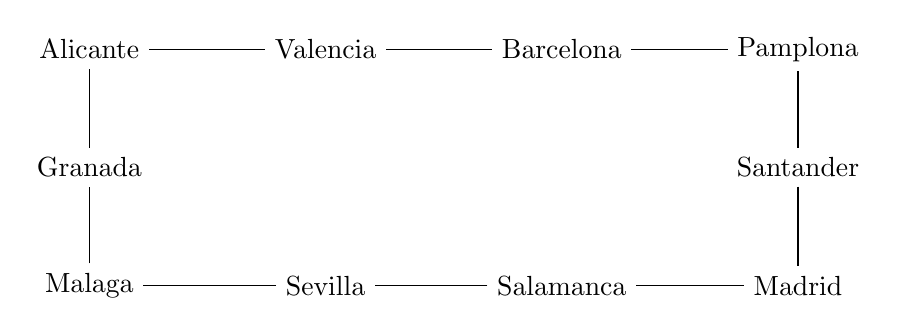
\begin{tikzpicture}
\node (a) at (0, 0) {Malaga};
\node (b) at (0, 1.5) {Granada};
\node (c) at (0, 3) {Alicante};
\node (d) at (3, 3) {Valencia};
\node (e) at (6, 3) {Barcelona};
\node (f) at (9, 3) {Pamplona};
\node (g) at (9, 1.5) {Santander};
\node (h) at (9, 0) {Madrid};
\node (i) at (6, 0) {Salamanca};
\node (j) at (3, 0) {Sevilla};
\draw (a)--(b)--(c)--(d)--(e)--(f)--(g)--(h)--(i)--(j)--(a);
\end{tikzpicture}
\caption{The fastest route around Spanish cities with the distances given in Table~\ref{tab:distance_matrix}.}
\label{fig:fastest_route_around_spannish_cities}
\end{center}
\end{figure}

\section{Algorithms}
\label{sec:Algorithms}

To solve the travelling salesman problem we implemented a variety of algorithms, which are detailed in ``The \texttt{TSP} algorithm suite'', which can be found at\footnote{At a later date a second version of this will be migrated to \href{https://github.com/oliversheridanmethven}{https://github.com/oliversheridanmethven}.}
\begin{center}
\href{https://github.com/InFoMM/TSP}{https://github.com/InFoMM/TSP}.
\end{center}

The algorithms which I implemented can be found in the user guide for the suite. They are detailed quite extensively there, and so for brevity we will only give a very brief outline of some here. We detail \verb|increasing_loop| and \verb|tsp_ip_cut_set_oliver|, which is a graph based algorithm and an integer programming algorithm respectively.

\subsection{\texttt{increasing\_loop}}
\label{subsec:increasing_loop}

This begins by randomly picking three nodes in the network\footnote{Networks with three or less nodes are trivial to solve.} and forming a sub-loop from these. Then for an arbitrary node which is not in the sub-loop, we calculate what would be the minimal deformation of the existing sub-loop that would include this additional node. We perform this assessment for each of the nodes not included in the sub-loop, and then whichever gives the minimum increase in the sub-loop's round trip distance, we include this node into the sub-loop. We perform this process iteratively until there are no remaining unconnected nodes. This algorithm is demonstrated in Figure~\ref{fig:increasing_loop}.

\begin{figure}[htb]
\centering
\begin{subfigure}{0.3\textwidth}
\centering
\fbox{\begin{tikzpicture}
\draw[fill] (0,0) circle (2pt) coordinate (a);
\draw[fill] (0.4,3) circle (2pt) coordinate (b);
\draw[fill] (2,3.4) circle (2pt) coordinate (c);
\draw[fill] (3.5,0.7) circle (2pt) coordinate (d);
\draw[fill] (1,1) circle (2pt) coordinate (e);
\draw[fill] (2,2) circle (2pt) coordinate (f);
\draw[fill] (3,0.7) circle (2pt) coordinate (g);
\end{tikzpicture}}
\caption{Initial configuration.}
\label{subfig:increasing_loop_step_0}
\end{subfigure}
\begin{subfigure}{0.3\textwidth}
\centering
\fbox{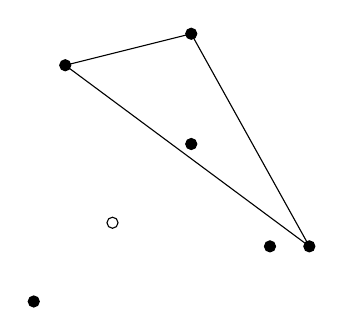
\begin{tikzpicture}
\draw[fill] (0,0) circle (2pt) coordinate (a);
\draw[fill] (0.4,3) circle (2pt) coordinate (b);
\draw[fill] (2,3.4) circle (2pt) coordinate (c);
\draw[fill] (3.5,0.7) circle (2pt) coordinate (d);
\draw[] (1,1) circle (2pt) coordinate (e);
\draw[fill] (2,2) circle (2pt) coordinate (f);
\draw[fill] (3,0.7) circle (2pt) coordinate (g);
\draw (b)--(d);
\draw (b)--(c);
\draw (c)--(d);
\end{tikzpicture}}
\caption{Initialisation.}
\label{subfig:increasing_loop_step_1}
\end{subfigure}
\begin{subfigure}{0.3\textwidth}
\centering
\fbox{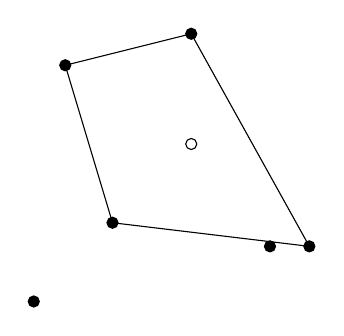
\begin{tikzpicture}
\draw[fill] (0,0) circle (2pt) coordinate (a);
\draw[fill] (0.4,3) circle (2pt) coordinate (b);
\draw[fill] (2,3.4) circle (2pt) coordinate (c);
\draw[fill] (3.5,0.7) circle (2pt) coordinate (d);
\draw[fill] (1,1) circle (2pt) coordinate (e);
\draw[] (2,2) circle (2pt) coordinate (f);
\draw[fill] (3,0.7) circle (2pt) coordinate (g);
\draw (b)--(e);
\draw (e)--(d);
\draw (b)--(c);
\draw (c)--(d);
\end{tikzpicture}}
\caption{First addition.}
\label{subfig:increasing_loop_step_2}
\end{subfigure}
\vspace{1ex}\\
\begin{subfigure}{0.3\textwidth}
\centering
\fbox{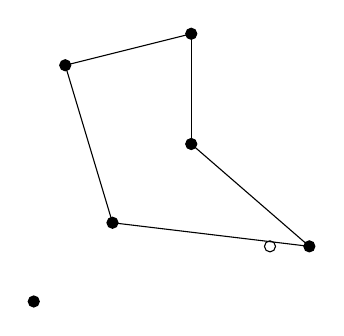
\begin{tikzpicture}
\draw[fill] (0,0) circle (2pt) coordinate (a);
\draw[fill] (0.4,3) circle (2pt) coordinate (b);
\draw[fill] (2,3.4) circle (2pt) coordinate (c);
\draw[fill] (3.5,0.7) circle (2pt) coordinate (d);
\draw[fill] (1,1) circle (2pt) coordinate (e);
\draw[fill] (2,2) circle (2pt) coordinate (f);
\draw[] (3,0.7) circle (2pt) coordinate (g);
\draw (b)--(e);
\draw (e)--(d);
\draw (b)--(c);
\draw (c)--(f);
\draw (f)--(d);
\end{tikzpicture}}
\caption{Intermediate addition.}
\label{subfig:increasing_loop_step_3}
\end{subfigure}
\begin{subfigure}{0.3\textwidth}
\centering
\fbox{\begin{tikzpicture}
\draw[] (0,0) circle (2pt) coordinate (a);
\draw[fill] (0.4,3) circle (2pt) coordinate (b);
\draw[fill] (2,3.4) circle (2pt) coordinate (c);
\draw[fill] (3.5,0.7) circle (2pt) coordinate (d);
\draw[fill] (1,1) circle (2pt) coordinate (e);
\draw[fill] (2,2) circle (2pt) coordinate (f);
\draw[fill] (3,0.7) circle (2pt) coordinate (g);
\draw (b)--(e);
\draw (b)--(c);
\draw (c)--(f);
\draw (f)--(d);
\draw (g)--(d);
\draw (g)--(e);
\end{tikzpicture}}
\caption{Final addition.}
\label{subfig:increasing_loop_step_4}
\end{subfigure}
\begin{subfigure}{0.3\textwidth}
\centering
\fbox{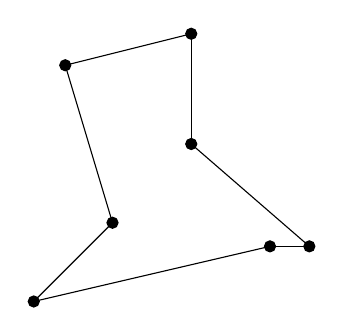
\begin{tikzpicture}
\draw[fill] (0,0) circle (2pt) coordinate (a);
\draw[fill] (0.4,3) circle (2pt) coordinate (b);
\draw[fill] (2,3.4) circle (2pt) coordinate (c);
\draw[fill] (3.5,0.7) circle (2pt) coordinate (d);
\draw[fill] (1,1) circle (2pt) coordinate (e);
\draw[fill] (2,2) circle (2pt) coordinate (f);
\draw[fill] (3,0.7) circle (2pt) coordinate (g);
\draw (b)--(e);
\draw (b)--(c);
\draw (c)--(f);
\draw (f)--(d);
\draw (g)--(d);
\draw (g)--(a);
\draw (e)--(a);
\end{tikzpicture}}
\caption{Final route.}
\label{subfig:increasing_loop_step_5}
\end{subfigure}
\caption{Progression of the increasing loop algorithm. Empty circles  represent the next global minimum for the next iteration.}
\label{fig:increasing_loop}
\end{figure}


\subsection{\texttt{tsp\_ip\_cut\_set\_oliver}}
\label{subsec:tsp_ip_cut_set_oliver}

We can represent the edges that connect any two cities $ i $ and $ j $ by a $ n \times n $ matrix $ x_{ij} $, taking values in $ \{0, 1\} $, which represent an edge being absent or present respectively. We impose the constraint that there is only one path in and out of a city by $ \sum_{i} x_{ij} = 1 \: \forall j $ and  $ \sum_{j} x_{ij} = 1 \: \forall i $. We then input this formulation into the Matlab \verb|intlinprog| solver where we request integer solutions.

The output produced might contain loops, so to prevent this, after the first iteration we form a constraint which ensures that we must form a connection between each of the sub-loops and the remaining points. We then iteratively add these constraints to the solver, at each stage eliminating some specific configuration of sub-loops, until there is only one global loop, which will be an optimal solution (not necessarily unique).

Extensions of this where we drop the no sub-loop constraint, and also integer solutions are detailed in the \texttt{TSP} algorithm suite.

\section{Performance}
\label{sec:performance}

We have two classes of algorithms, those which compute exact solutions, and those which compute approximate solutions. Those which compute exact solutions are accurate but may take a long time to execute, whereas the approximate solutions may be quick to run, but may give routes which are not optimal (although possibly close to optimal). With any algorithm a compromise between execution time and accuracy has to be met, and so  depending on the need of the user, we present some characteristics of the algorithms available.

\subsection{Execution times}
\label{subsec:execution_times}

We benchmark the average execution time of algorithms on the Spanish data set from Table~\ref{tab:distance_matrix} over 100 trials. Furthermore, generating random symmetric distance matrices of various sizes, we can see how the algorithms scale with the number of cities. The results are summarised  in Table~\ref{tab:execution_times}.


\begin{table}[htb]
\footnotesize
\begin{center}
\begin{tabular}{|L{0.3\textwidth}|c@{\hspace{1ex}}|c@{\hspace{1ex}}c@{\hspace{1ex}}c@{\hspace{1ex}}c@{\hspace{1ex}}c@{\hspace{1ex}}c@{\hspace{1ex}}c@{\hspace{1ex}}|}
\hline
\multicolumn{1}{|c|}{Algorithm}          & Spain & 6 & 8 & 10 & 12 & 15 & 20 & 30 \\ \hline
\texttt{increasing\_loop}                &   $ 1.6 \! \cdot \! 10^{-4} $   & $ 2.2  \! \cdot \! 10^{-4} $ & $ 1.0  \! \cdot \! 10^{-4} $ & $ 1.0  \! \cdot \! 10^{-4} $ & $ 1.4 \! \cdot \!10^{-4} $ & $ 1.8 \! \cdot \! 10^{-4} $ & $ 2.7 \! \cdot \! 10^{-4} $ & $ 8.5 \! \cdot \! 10^{-4} $ \\
\texttt{forcefully\_increasing\_loop}    &  $ 3.1 \! \cdot \! 10^{-4}$  & $ 6.7 \! \cdot \! 10^{-5}$ &  $ 9.6 \! \cdot \! 10^{-5}$ &  $ 9.1 \! \cdot \! 10^{-5}$ &  $ 1.3 \! \cdot \! 10^{-4}$ &  $ 1.7 \! \cdot \! 10^{-4}$ &  $ 7.2 \! \cdot \! 10^{-4}$ &  $ 4.6 \! \cdot \! 10^{-4}$ \\
\texttt{tsp\_ip\_cut\_set\_oliver.m}     &    $ 5.7 \! \cdot \! 10^{-1}$   &  $ 9.1 \! \cdot \! 10^{-2}$ &  $ 2.0 \! \cdot \! 10^{-1}$ &  $ 1.8 \! \cdot \! 10^{0}$ &  \textasteriskcentered &\textasteriskcentered & \textasteriskcentered & \textasteriskcentered \\
\texttt{tsp\_ip\_no\_cut\_set\_oliver.m} &    $ 2.1 \! \cdot \! 10^{-2}$    & $ 1.1 \! \cdot \! 10^{-2}$  & $ 1.1 \! \cdot \! 10^{-2}$  & $ 1.1 \! \cdot \! 10^{-2}$  & $ 1.1 \! \cdot \! 10^{-2}$  & $ 1.4 \! \cdot \! 10^{-2}$  & $ 1.5 \! \cdot \! 10^{-2}$  & $ 1.6 \! \cdot \! 10^{-2}$  \\
\texttt{tsp\_lp\_no\_cut\_set\_oliver.m} &  $ 1.7 \! \cdot \! 10^{-2}$   & $ 1.1 \! \cdot \! 10^{-2}$ & $ 1.2 \! \cdot \! 10^{-2}$ & $ 1.4 \! \cdot \! 10^{-2}$ & $ 2.1 \! \cdot \! 10^{-2}$ & $ 2.1 \! \cdot \! 10^{-2}$ & $ 2.9 \! \cdot \! 10^{-2}$ & $ 3.4 \! \cdot \! 10^{-2}$ \\ \hline
\end{tabular}
\end{center}
\caption{Execution times in seconds of various algorithms for the Spanish data set and randomly generated data. Entries marked with \textasteriskcentered{} indicate when the algorithms run out of memory.}
\label{tab:execution_times}
\end{table}

Looking at the results here we see that for the \verb|increasing_loop| algorithm, the performance does not change much on this problem scale, suggesting that the problems are not large enough to be the rate limiting step. Notice further that this is relatively very fast, and typically takes no more than 5 or 10 runs on the Spanish data set to find the optimal solution.

Conversely we can see that the \verb|tsp_ip_cut_set_oliver| is very slow, and while exact, quickly encounters memory issues and has poor scaling.

\subsection{Comparison to optimality}
\label{subsec:comparison_to_optimality}

To see how accurate our algorithms are, we need to know what the optimal solution is. We present in Table~\ref{tab:optimality} the average fractional discrepancy error from optimality for the Spanish cities example from Table~\ref{tab:distance_matrix}.

\begin{table}[htb]
\begin{center}
\begin{tabular}{|L{0.4\textwidth}|c|}
\hline
\multicolumn{1}{|c|}{Algorithm}          & Error \\ \hline
\texttt{increasing\_loop}                &   5.7   \\
\texttt{forcefully\_increasing\_loop}    &   3.2   \\
\texttt{tsp\_ip\_cut\_set\_oliver.m}     &   -   \\
\texttt{tsp\_ip\_no\_cut\_set\_oliver.m} &   -13.6   \\
\texttt{tsp\_lp\_no\_cut\_set\_oliver.m} &   NA   \\ \hline
\end{tabular}
\end{center}
\caption{The relative error of various algorithms measured against the exact solution to the Spanish data. Negative entries indicate solutions with shorter distances (contain sub-loops), and entries marked NA give non physical routes such as those with partial edges.}
\label{tab:optimality}
\end{table}

Looking at the results from Table~\ref{tab:optimality}, we see that the \verb|increasing_loop| algorithm seems to give reasonable performance. More interestingly though, while \verb|tsp_ip_cut_set_oliver| is exact, its extension that allows sub-loops gives a shorter round trip distance. Additionally the linear programming relaxation gives partial paths between cities, and so the route is unphysical and has an undefined distance. 

\section{Conclusion}
\label{sec:conclusion}

Having seen the performance of the various schemes, we see that for large numbers of cities exact solvers are completely infeasible either due to memory constraints or infeasible execution times. The graph based solvers typically either try to enumerate all possible paths and quickly become undesirable, or have some form of greedy progression which can give a route in feasible time which can be expected to be near optimal.

Conversely we have seen we can pose the problem as an integer programming optimisation, but most solvers struggle to produce a solution with a continuous path. Relaxations for linear solvers are quicker and more convergent, but typically give non-physical solutions with partial paths between cities. 

\clearpage
\bibliography{references}
\end{document}